%!TEX root = ../main.tex

%!TEX root = ../main.tex

\chapter{Einleitung}
Angesichts des Klimawandels sind umweltschonende Fortbewegungsmittel besonders wichtig. Insbesondere Elektrofahrzeuge spielen eine zentrale Rolle bei der Reduktion von CO2-Emissionen und einer nachhaltigeren Mobilität \cite{urlIdParisKlimaabkommen}. Dafür müssen Elektrofahrzeuge langlebig sein, da die Produktion sehr ressourcenaufwendig ist \cite{urlIdUmwelteinflussLithiumBatterien}. Um die Lebensdauer realistisch abzuschätzen, sind genaue Vorhersagen zur Batteriealterung notwendig. Mit ihnen kann eine nachhaltigere Batterieentwicklung umgesetzt und das Vertrauen in Elektrofahrzeuge gestärkt werden.\\
Die Lebensdauer einer Batterie hängt sowohl vom Batterietyp, etwa Li-Ion- oder Festkörperbatterien \cite{urlIdBatterieAlterungLithiumBatterien}, \cite{urlIdBatterieAlterungVerschiedenerSoCLithiumBatterien}, \cite{urlIdBatterieAlterungFestkörperBatterien}, \cite{urlIdBatterieAlterungVerschiedenerSoCLithiumBatterien}, als auch vom Nutzungsprofil, das durch Fahrverhalten und Klimabedingungen beeinflusst wird \cite{urlIdBatterieAlterungTemperatur}, ab. Zudem ist die Vorhersage der Batteriealterung bei Flottenfahrzeugen häufig durch verrauschte und unvollständige Datensätze erschwert.\\
Diese Arbeit widmet sich der datengetriebenen Vorhersage der Batteriealterung von elektrischen Kundenfahrzeugen. Dabei werden Machine-Learning- und Time-Series-Forecasting-Algorithmen analysiert und hinsichtlich Genauigkeit und Praxistauglichkeit validiert.

\pagebreak
\section{Problemstellung}
Trotz identischer Batterien beeinflussen das individuelle Fahr- \cite{urlIdBatterieAlterungVerschiedenerSoCLithiumBatterien} und Ladeverhalten \cite{urlIdBatterieAlterungVerschiedenerSoCLithiumBatterien} sowie Umweltbedingungen \cite{urlIdBatterieAlterungTemperatur} den Alterungsprozess erheblich, wodurch eine verlässliche Lebensdauerprognose über Jahre hinweg komplex und unsicher wird. Diese Unsicherheit erhöht sich durch unvollständige, verrauschte Flottendaten \cite{idEigeneFlottenDaten} und unbekanntes zukünftiges Fahrverhalten zusätzlich.\\
Physikalisch-chemische Modelle bieten zwar präzise Alterungssimulation im Labor \cite{urlIdPhysicalAgingMethodsForLIBs}, sind jedoch aufgrund aufwändiger Modellierung, Parametrierung und Validierung kaum auf Flotten skalierbar. Datengetriebene Ansätze, wie maschinelles Lernen und neuronale Netze \cite{urlIdDataAgingMethodsForLIBs}, sind skalierbar, jedoch anfällig für verrauschte Daten und Überanpassung.\\
Damit erweist sich die Prognose der Batteriealterung von einzelnen Fahrzeugen in der Fahrzeugflotte als komplex, da Modellauswahl und Datenlage ihr eigenes Maß an Unsicherheit mit sich bringen. Um die gesamten Flottendaten bei der Alterungsprognose mit einzubeziehen, beschäftigt sich diese Arbeit mit dem datengetriebenen Ansatz.

\pagebreak
\section{Ziel der Arbeit}
Das Ziel dieser Arbeit ist die Integretation eines bestehenden Algorithmus zur Prognose der Batteriealterung in Elektrofahrzeugen, basierend auf realen Fahrzeugflottendaten. Der Fokus liegt dabei auf der Zeitreihenvorhersage des Batterie-Gesundheitszustands über mehrere Jahre für einzelne Fahrzeuge. Präzise Prognosen tragen zur verbesserten Bewertung des Gesundheitszustands bei und ermöglichen eine nachhaltigere Nutzung der Batterien.
\\
Die Grundlage der Vorhersagen bilden die Fahrzeugflottendaten, die typischerweise Rauschen, Ungenauigkeiten und Messlücken aufweisen \cite{idEigeneFlottenDaten}. Mit synthetischen Daten können diese Probleme minimiert werden, jedoch sind die generierten Daten kaum validierbar. Daher verzichtet die Arbeit bewusst auf die Verwendug synthetischer Daten.
\\
Zur Zielerreichung werden Batterieaufbau sowie relevante Alterungsprozesse untersucht, um letztere mittels datengetriebener Modellen wie Machine Learning und neuronalen Netzen vorherzusagen. Die Datenaufbereitung vor dem Modelltraining umfasst die Bereinigung des bestehenden Datensatzes von Ausreißern und Messlücken sowie der Identifikation der wichtigsten Einflussfaktoren auf die Alterung. Beim Training des Algorithmus führen Überanpassung (Overfitting) und Modellwahl zu Unsicherheiten. Ersteres entsteht besonders bei kleinen oder stark korrelierten Datensätzen, sodass das Modell Details statt Muster erlernt und nicht robust gegenüber neuen Daten ist. Letzeres beschreibt, dass unterschiedliche Modelle (z.B. RNN, LSTM, GPR, XGBoost) unterschiedlich stark auf Datenmängel und verrauschten Daten reagieren. Die geeignete Wahl der Modelle wird in Kapitel 2 dargelegt.
Die Validierung der Modellergebnisse erfolgt anhand typischer Degradationsmuster von \ac{LIB} aus der Literatur, um realitätsnahe Ergebnisse zu liefern. Dabei grenzt sich die Arbeit bewussst von physikalsisch-chemischen Modellierungen und Laboruntersuchungen ab. (Wie kann ich stattdessen die Modellergebnisse validieren: Expertenwissen? Physikalisch Modelle als Referenz?)
\\
Der Erfolg des entwickelten Verfahrens wird abschließend anhand Fehlermaßen wie RMSE oder MAE sowie die Robustheit gegenüber verrauschten und unvollständigen Daten und die Fähigkeit zur Generalisierung auf unterschiedliche Fahrzeugprofile innerhalb der Flotte bewertet.
\pagebreak
\section{Vorgehensweise}
\paragraph{Disclaimer} In zukünftigen Version bindet das Kapitel Ziel der Arbeit die Strukturierung als Fließtext ein.
 
\begin{itemize}
    \item \textbf{Theoretische Grundlage}: Ausführung der theoretischen Grundlagen der Batteriealterung.
    \item \textbf{Modellanalyse}: Auswahl und Analyse geeigneter Machine-Learning- und Zeitreihen-Algorithmen.
    \item \textbf{Datenanalyse}: Untersuchung der Fahrzeugflottendatten hinsichtlich Qualität, Rauschen und Ausreißer.
    \item \textbf{Feature-Identifikation}: Identifikation relevanter Features für die Batteriealterung.
    \item \textbf{Datenvorverarbeitung}: Vorverarbeitung und Filtern der Fahrzeugflottendaten.
    \item \textbf{Modelltraining und -validierung}: Training und Validierung der Modelle anhand bekannten Alterungsverläufen.
    \item \textbf{Bewertung}: Vergleich der Modellergebnisse unter Berücksichtigung von Genauigkeit, Robustheit und Generalisierbarkeit.
\end{itemize}


%!TEX root = ../main.tex

\chapter{Aufbau und Alterung von Fahrzeugbatterien}
Elektrofahrzeuge nutzen überwiegend Lithium-Ionen-Batterien (LIB), die sich in Größe, Bauform und der chemischen Zusammensetzung ihrer Komponenten unterscheiden. Eine zentrale Rolle für die Leistungsfähigkeit der Batterie spielt die Kathode. Die hierfür eingesetzten Materialen bestimmen maßgeblich Energiedichte, Lade- und Entladeleistung sowie Lebensdauer. Obwhol der Begriff "Zellchemie" streng genommen die Gesamtheit aller elektrochemisch relevanten Materialen umfasst - einschließlich Anode, Elektrolyt und Separator - wird in der Praxis häufig nur die Zusammensetzung der Kathode bezeichnet. In Elektrofahrzeungen kommen vor allem drei Kathodenmaterialen zum Einsatz: Lithium-Eisenphosphat (LFP, \ce{LiFePO4}),  Lithium-Nickel-Mangan-Cobalt (NMC, \ce{LiNiMnCoO2}) und Lithium-Nickel-Cobalt-Aluminium (NCA, \ce{LiNiCoAIO2}). LFP zeichnet sich durch eine lange Lebensdauer und eine hohe thermische Stabilität aus, weist jedoch im Vergleich zu NMC- und NCA-Technologien eine geringere Energiedichte auf. Letztere ermöglichen eine höhere Energiedichte, gehen jedoch mit einer geringeren thermischen Stabilität einher. NMC-Zellen werden anhand ihres Massenverhältnis von Nickel, Mangan und Cobalt klassifiziert, z.B. als NMC111, NMC622 oder NMC811. Die Zahlen geben die prozentuale Zusammensetzung der Metalle an - eine NMC622-Zelle enthält etwa 60\% Nickel, 20\% Mangan und 20\% Cobalt. Ein erhöhter Nickelanteil sorgt für eine bessere Energiedichte, jedoch zulasten der Lebensdauer. Diese Zellchemien finden Einsatz in unterschiedlichen Bauformen, wie Pouch- oder Zylinderzellen \ref{fig:pouch-zylinder-zelle}. 
\begin{figure}[H]
	\centering
	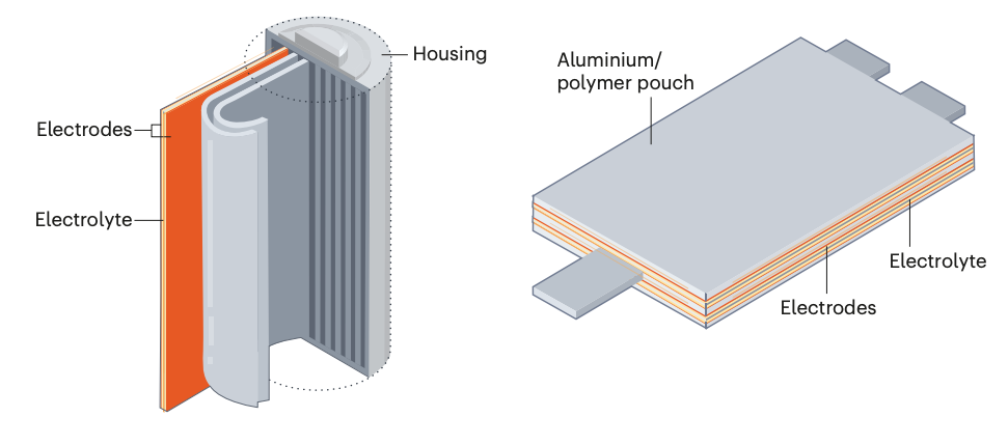
\includegraphics[height=0.25\linewidth]{resources/images/pouch-zylinder-zelle}
	\caption{Beispiel einer Pouch- und einer Zylinderzelle}
	\label{fig:pouch-zylinder-zelle}
\end{figure}
Pouch-Zellen bieten eine hohe Energiedichte und lassen sich flexibel an unterschiedliche Bauformen anpassen. Während des Alterungsprozesses neigen sie jedoch zur Expansion, was die Batteriealterung beschleunigt \cite{articlePouchZellenAlterung}. Hingegen zeichnen sich Zylinderzellen durch eine lange Lebensdauer und eine robuste Bauform aus. Dafür ist Kühlung bei Rundzellen aufwendiger und die Energiedichte bei gleichem Bauvolumen oftmals geringer.

\section{Hauptbestandteile von LIB und ihre Funktionen}
Eine LIB besteht aus Kathode, Anode, Elektrolyt, Separator, Stromkollektoren und Bindemittel \cite{urlIdAufbauBatterie}, wie in Abbildung \ref{fig:aufbau-nmc-zelle} dargestellt. 
\begin{figure}[H]
	\centering
	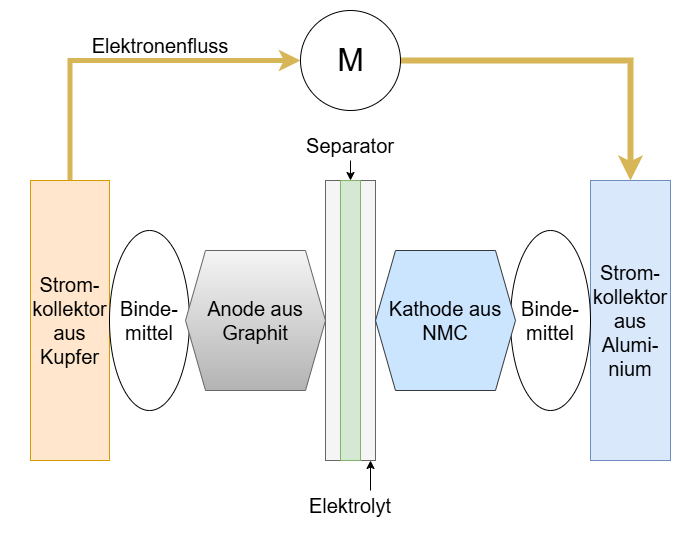
\includegraphics[height=0.4\linewidth]{resources/images/aufbau-nmc-zelle}
	\caption{Aufbau einer LIB-Zelle beim Entladeprozess \cite{articleAlterungLithiumBatterien}}
	\label{fig:aufbau-nmc-zelle}
\end{figure}

An der Kathode findet die Oxidation und Deinterkalation von \ce{Li+}-Ionen, während an der Anode die Oxidation und die Interkalation von \ce{Li+}-Ionen erfolgt. Das Elektrolyt ermöglicht den Transport von diesen \ce{Li+}-Ionen zwischen Anode und Kathode. Der Separator lässt Ionen, jedoch keine Elektronen passieren. Dadurch unterbindet er den direkten Kontakt der Elektroden, der zu einem Kurzschluss führen würde. Die Stromkollektoren sorgen für eine leitfähige Verbindung zwischen Elektrodenmaterial und äußerem Stromkreis, sodass Elektronen effizient abgeleitet werden. Die Bindemittel fixieren Anode und Kathode an ihrem jeweiligen Stromkollektor und gewährleisten Stabilität beim Lade- und Entladeprozess.

Entladung
Beim Entladevorgang deinterkaliert Lithium aus der Graphitstruktur der Anode und oxidiert zu einem \ce{Li+}-Ion unter Abgabe eines Elektrons. Dieses Elektron fließt über den Stromkollektor aus Kupfer zur Kathode, wo es Cobaltionen (\ce{Co^{3+}}) in der NMC-Kathode zu \ce{Co^{2+}} reduziert. Parallel dazu diffundiert das \ce{Li+}-Ion über das Elektrolyt und interkaliert sich in der Kristallstruktur der Kathode. Die zugrunde liegende Reaktion lässt sich vereinfacht wie folgt darstellen:
\begin{align*}
    \ce{Li &-> Li+ + e-}              &\quad& \text{(Oxidation beim Entladeprozess)} \\
    \ce{Co^{3+} + e- &-> Co^{2+}}     &\quad& \text{(Reduktion beim Entladeprozess)} \\
    \ce{Li + Co^{3+} &<=> Li^+ + Co^{2+}} &\quad& \text{(Redoxreaktion)}
\end{align*}

Beim Ladeprozess kehrt sich der Redoxprozess um und Anode und Kathode tauschen ihre räumliche Position. Das Cobalt an der Anode oxidiert und \ce{Li+}-Ionen deinterkalieren aus der Kristallstruktur. Die dabei abgegebenen Elektronen fließen vom Aluminium-Stromkollektor über den externen Stromkreis zum Kupfer-Stromkollektor zurück. Zeitgleich transportiert das Elektrolyt die \ce{Li+}-Ionen zur Graphitstruktur, wo die Interkalation stattfindet.
Die Alterungsmechanismen der Batterien stören diese zuvor erläuterten Prozesse, wodurch sich Batterieleistung und -kapazität verringern. Durch eine Analyse dieser Mechanismen lassen sich die wichtigsten Einflussfaktoren identifizieren. Insbesondere diese Faktoren sollten im Datensatz für das Training der datengetriebenen Modelle berücksichtigt werden, da nicht-relevante Parameter Unschärfe und Ungenauigkeiten in den Lernprozess einbringen. Dies ermöglicht eine genaue Vorhersage der Batterialterung. Deshalb beleuchten die nächsten Kapitel die Zusammenhänge zwischen Alterungsmechanismen und Einflussfaktoren.

\section{Alterung von Batterien}
Die Alterung von Batterien beschreibt den fortschreitenden Verlust von Leistung und Kapazität. Sie lässt sich in kalendarische und zyklische Alterung unterteilen. Kalendarische Alterung erfolgt zeitabhängig und unabhängig von Ladezyklen, während zyklische Alterung primär durch Lade- und Entladeprozessen bedingt ist. Beide Alterungsformen lassen sich auf dieselben grundlegenden Mechanismen zurückführen: dem Verlust aktiven Lithiums, dem Abbau des aktiven Elektrodenmaterials, dem Rückgang des Elektrolyts und der Erhöhung des internen Widerstands.
Der Verlust des aktiven Lithiums (engl. loss of lithium, (LLI)) reduziert die Menge an verfügbaren \ce{Li+}-Ionen. Diese Ionen sindfür den inneren Ionenstromkreis verantwortlich, der den Elektronenfluss im äußeren Stromkreis ermöglicht. Ohne ausreichend \ce{Li+}-Ionen können weniger Elektronen im äußeren Stromkreis fließen, was Leistung und Kapazität der Batterie limitiert.\\
Der Verlust des aktiven Materials von Kathode und Anode verschlechtert die Ein- und Auslagerung von \ce{Li+}-Ionen und Elektronen. Das schränkt den Ionen- und Elektronenfluss ein, was zur Reduktion von Leistung und Kapazität führt.\\
Der Verlust des aktiven Materials an Kathode und Anode verschlechtert Interkalation und Deinterkalation von \ce{Li+}-Ionen und Elektronen, welche den Ionen- und Elektronenfluss ermöglichen. Eine Störung dieses Prozesses verringtert Leistung und Kapazität.\\
Der Verlust von Elektrolyt verringert den Transport von \ce{Li+}-Ionen zwischen Kathode und Anode, was den Ionenfluss beeinträchtigt. Dies führt zu einem geringeren Elektronenfluss und einer Minderung von Leistung und Kapazität. Häufig geht der Elektrolytabbau mit einem  Verlust von Lithium und aktiven Material einher.\\
Ein erhöhter interner Widerstand fördert die Wärmeentwicklung, wodurch die anderen Alterungsprozesse beschleunigt werden. Gleichzeitig führt er zu Spannungsabfällen, was die nutzbare Kapazität reduziert.
Diese Mechanismen interagieren miteinander und werden durch interne sowie externe Prozesse beeinflusst. Eine Analyse der internen Prozesse ist erforderlich, um den Einfluss externen Faktoren auf die Batteriealterung zu verstehen. Letztere misst meist das Batterie-Management-System (BMS), was die Datengrundlage für das Training der Modelle darstellt.

\subsection{Interne Faktoren}
\paragraph{SEI} Bereits bei den ersten Ladezyklen bildet sich an der Grenzfläche zwischen Anode und Elektrolyt eine irreversible Grenzschicht, das sogennante Solid Electrolyte Interface (SEI). Sie entsteht durch Reduktionsreaktionen des Elektrolyten an der Anodenoberfläche. Im Zuge dieser Reaktionen werden Lithium-Ionen irreversibel gebunden, wodurch sie dem elektrochemischen Prozess nicht mehr zur Verfügung stehen. Die SEI-Schicht blockiert den Durchtritt von Elektronen, lässt jedoch Ionen passieren. Mechanische Spannungen, wie die Expansion und Kontraktion der Graphitstruktur, führen zu Risse in der SEI-Schicht. Sie regeneriert diese Instabilitäten unter Einbindung von \ce{Li+}-Ionen, wodurch sie verdickt. Der fortschreitende Verlust an Lithium (LLI) sowie der Anstieg des internen Widerstands (IR) reduzieren die nutzbare Kapazität und beschleunigen den Alterungsprozess. Die Bildung der SEI-Schicht erklärt den anfänglich Abfall der Batteriekapazität bei LIB.

\paragraph{Kathode} Die Kathode dient als Quelle für \ce{Li+}-Ionen, die beim Entladen interkaliert werden. Während zyklischer Lade- und Entladevorgänge unterliegt die Kathodenstruktur mechanischen Spannungen durch Expansion und Kontraktion, was zur Bildung von Mikrorissen, Partikelablösung (Peeling) und strukturellem Zerfall führt. Zusätzlich kann es zur Auflösung von Übergangsmetallionen wie \ce{Ni^{2+}}, \ce{Co^{2+}} und \ce{Mn^{2+}} kommen, die durch den Separator zur Anode diffundieren und dort die SEI-Schicht destabilisieren. Dies trägt zur Kapazitätsreduktion (LLI, LAM) bei und erhöht den internen Widerstand (IR).
An der Kathodenoberfläche lagern sich bei elektrochemischen Reaktionen Abbauprodukte des Elektrolyten ab. Diese führen zur Bildung eines stabilen festen Grenzfilms – des sogenannten Cathode Electrolyte Interface (CEI). Das CEI schützt zwar die Kathode vor weiterer Elektrolyt-Zersetzung und reduziert den irreversiblen Materialverlust, wird jedoch mit zunehmender Zyklenzahl dicker und trägt dadurch ebenfalls zu einem Anstieg des IR bei.
Darüber hinaus kann sich die Verbindung zwischen Aktivmaterial und Stromkollektor durch thermische Belastung, elektrochemische Korrosion und mechanischen Stress lösen. Diese Degradation beschleunigt den Verlust aktiver Flächen und somit den Alterungsprozess der Batterie.
\paragraph{Elektrolyt und Stromkollektoren} Das Elektrolyt spielt eine zentrale Rolle im Transport von \ce{Li+}-Ionen zwischen den Elektroden. Dabei wird zwischen flüssigen, gelartigen und festen Elektrolyten unterschieden. Während der Lade- und Entladezyklen kommt es zu Redoxreaktionen zwischen Elektrolyt und Elektroden, wodurch die Bildung von SEI und CEI auf der Anode bzw. Kathode initiiert wird. Mit der fortschreitenden Nutzung wird das Elektrolyt zunehmend konsumiert, was zu einem kontinuierlichen Abbau und Neubildung dieser Grenzschichten führt. Die sich verdickenden Filme erhöhen den internen Widerstand (IR) und tragen somit zur Degradation der Batterie bei. Zudem wird bei der Elektrolyt-Dekomposition eine erhebliche Menge an Gas freigesetzt, was zu einer Volumenexpansion der Zelle führt. Die abgebauten Produkte lagern sich am Separator ab, was den \ce{Li+}-Ionen-Transport behindert und die Alterung der Batterie beschleunigt.
Die Stromkollektoren sind für die Sammlung der Elektronen an den Elektroden verantwortlich. Sie sind jedoch anfällig für Korrosion und Oxidation bei höheren Potentialen. Wird die Batterie überladen, kann die Graphit-Anode überschüssige \ce{Li+}-Ionen freisetzen, wodurch die Spannung das Auflösungspotential von Kupfer überschreitet. Dies führt zu einer Oxidation des Kupfers zu Kupferionen, die sich im Elektrolyten lösen. In den nachfolgenden Ladezyklen lagern sich diese Kupferionen an der Anodenoberfläche ab, was zu Kapazitätsverlust führt. Bei sehr hohen Spannungen kann es auch zu lokalisierten Korrosionsprozessen im Aluminium-Stromkollektor der Kathode kommen, was den IR weiter erhöht und die Batteriealterung beschleunigt.
\paragraph{Separator und Dendritenbildung}

Der Separator dient als Barriere, die den Durchtritt von Elektronen verhindert und ausschließlich den Transport von \ce{Li+}-Ionen ermöglicht. Er weist eine poröse Struktur auf, die unter normalen Bedingungen eine effiziente Ionenmigration sicherstellt. Wenn der Separator jedoch mit dem Elektrolyten reagiert, wird seine Integrität beeinträchtigt. Dies führt zur Bildung von Gasen während der Elektrolyt-Zersetzung, was eine Volumenexpansion der Batterie zur Folge hat und den mechanischen Stress erhöht. Der Separator wird dadurch zunehmend beschädigt, was die Alterung der Batterie beschleunigt.

Zusätzlich lagern sich Dekompositionsprodukte der Anode und Kathode an der Oberfläche des Separators ab. Diese Ablagerungen blockieren die Poren und verringern die Ionenmigration, was zu einer verminderten Migrationsrate von \ce{Li+}-Ionen führt und die Leistung der Batterie weiter verschlechtert. Ein weiterer kritischer Faktor ist die Bildung von Lithium-Dendriten, die durch Lithium-Plating entstehen und den Separator durchdringen können. Dies beschleunigt die Alterung der Batterie erheblich und kann im schlimmsten Fall zu internen Kurzschlüssen führen. Hohe Temperaturen verstärken diesen Prozess, da sie den Separator zum Schrumpfen bringen und die Porengröße verringern oder sogar vollständig blockieren, was die Ionenleitung weiter hemmt.



\subsection{Externe Faktoren}

Die wesentlichen externen Faktoren, die die Batteriealterung beschleunigen, umfassen den Ladezustand (State of Charge, SoC), die Tiefenentladung (Depth of Discharge, DOD), die Lade-Entlade-Rate und die Temperatur.

Mit SoC ist das Verhältnis zwischen dem aktuellen Ladezustand und der maximalen Kapazität einer Batterie gemeint. Es besteht eine enge Verbindung zwischen dem SoC und der Batteriespannung, da Änderungen im Ladezustand die Cut-Off-Spannung der Batterie beeinflussen. Ein hoher SoC führt zu einer Erhöhung der Spannung an der positiven Elektrode und einer Reduktion der Spannung an der negativen Elektrode. Dies kann die Stabilität der positiven Elektrode beeinträchtigen und zu deren Ablösung führen, was eine Expansion und Interkalation von \ce{Li+}-Ionen zur Folge hat. Dieser Prozess begünstigt die Rissbildung am Solid Electrolyte Interface (SEI) und deren Regeneration, was zu einer Zunahme des Lithium-Ionen-Verlusts (LAM) führt. Ein hoher SoC fördert zudem die Gasbildung an der positiven Elektrode, was zu struktureller Degradation, mechanischer Ermüdung und Partikelfraktur führt, was letztlich den Kapazitätsverlust beschleunigt. Andererseits führt ein niedriger SoC zur Auflösung von Kupfer an der Anode, was den Lithium-Ionen-Verlust (LLI) und den internen Widerstand (IR) erhöht.

Das Batterie-Management-System (BMS) misst kontinuierlich den SoC und sorgt dafür, dass die Batterie innerhalb sicherer Grenzen betrieben wird. Im Vergleich zur Lagerung bei 100\% SoC bildet sich bei einem SoC von etwa 50\% eine stabilere SEI-Schicht, was die Lebensdauer der Batterie verlängert.

Mit DOD ist der Anteil der Kapazität gemeint, der im Vergleich zur vollen Kapazität der Batterie entladen wurde. Ein höherer DOD fördert die Freisetzung von \ce{Li+}-Ionen und beschleunigt die Zersetzung des Elektrolyten. Ein niedriger DOD verursacht hingegen eine größere Volumenänderung der aktiven Materialien während des Lade- und Entladezyklus, was zusätzlichen mechanischen Stress auf die Batterie ausübt. Dies führt zu Rissen in den Elektroden und beschleunigt die Alterung. Ein tieferer DOD ist oft mit einer höheren Betriebstemperatur verbunden, was die thermische Degradation weiter verstärken kann. Während des Zyklusprozesses wird die Graphitanode bei hohen DODs ausgedehnt, wodurch sich der Abstand zwischen den Graphitschichten vergrößert. Dies führt dazu, dass das schichtgelagerte Graphit freigelegt wird und mehr Oberfläche dem Elektrolyten ausgesetzt wird, was die vollständige Interkalation von \ce{Li+}-Ionen begünstigt. Bei \ce{LiFePO4}-Batterien wurde eine erhöhte Alterungsrate festgestellt, wenn der DOD tiefer und häufiger war, auch bei gleicher Zyklenzahl.


insert: SEM image of battery components after different DOD over-discharge cycles. Helle weiße PArtikel indiziren die Bildung von Kupfer. Höherer DOD over-discharge -> mehr weiße Partikel -> mehr Kupfer Deposition.

\subsection{Externe Faktoren}

\subsubsection{Tiefenentladung und Separatorstruktur}

Bei einer Tiefenentladung von über 100 % DOD, insbesondere bei 112,5 % DOD, verformt sich die poröse Struktur des Separators erheblich. Die meisten Poren sind entweder verstopft oder sogar vollständig verschlossen. Dies ist auf die Zersetzung des Anodenmaterials und die Ablagerung dieser Zersetzungsprodukte auf der Separatoroberfläche zurückzuführen, wodurch die Poren blockiert werden. Infolgedessen ist die Diffusion von \ce{Li+}-Ionen während der Zyklusprozesse stark eingeschränkt, was zu einem erhöhten inneren Widerstand führt und die Batteriealterung beschleunigt.

\subsubsection{Lade- und Entladerate (C-Rate)}

Die Lade- und Entladerate, auch als C-Rate bezeichnet, beschreibt den auf die Nennkapazität des Akkus bezogenen Lade- oder Entladestrom in Amperestunden. Eine hohe C-Rate bedeutet, dass der Akku intensiver belastet wird, was zu einer höheren Migration von \ce{Li+}-Ionen führt und die Zersetzung des Elektrolyten beschleunigt. Diese Zersetzung führt zu strukturellen Schäden an den Anoden- und Kathodenmaterialien. Hohe Ströme verursachen zudem eine lokale Überhitzung der Batteriematerialien, was zu einer Deformation der Struktur führt und die Interkalation bzw. Deinterkalation von \ce{Li+}-Ionen beeinträchtigt. Dies beschleunigt die Batteriealterung. Beispielsweise zeigt sich bei NMC622-Zellen, dass sich bei verschiedenen C-Raten unterschiedliche Zusammensetzungen der SEI-Schicht an der Graphitanode bilden. Gleichzeitig kommt es zu Lithium-Plating und weiteren Nebenreaktionen, die zu einem Lithium-Ionen-Verlust (LLI) führen.

\subsubsection{Temperatur}

Lithium-Ionen-Batterien (LIB) leisten am besten bei Temperaturen zwischen 15 und 35 °C. Extrem hohe oder niedrige Temperaturen wirken sich negativ auf die Leistung der Batterie aus. Bei hohen Temperaturen zersetzt sich der Elektrolyt schneller, und die Struktur von Anode und Kathode verändert sich, was die Alterung der Batterie beschleunigt. Niedrige Temperaturen hingegen reduzieren die Mobilität von \ce{Li+}-Ionen und die Aktivität des Elektrolyten, was die Effizienz von Lade- und Entladevorgängen einschränkt. Studien zeigen, dass hohe Temperaturen vor allem die Kathode betreffen, während niedrige Temperaturen Auswirkungen auf die Anode haben. Bei Lade- und Entladevorgängen bei hohen Temperaturen verstärkt sich die Bildung des Cathode Electrolyte Interface (CEI)-Films an der Kathode, was den internen Widerstand (IR) erhöht. Zudem entstehen Mikrorisse an der Kathode, was die Leitfähigkeit der Batterie reduziert und die Interkalation bzw. Deinterkalation von \ce{Li+}-Ionen verhindert, was wiederum die Kapazität negativ beeinflusst. Bei niedrigen Temperaturen reagiert das Elektrolyt mit den metallischen \ce{Li+}-Ionen an der Anode und bildet einen zweiten SEI-Film, was zu einem weiteren Lithium-Ionen-Verlust (LLI) führt.

\section{Zusammenfassung}

Zusammenfassend lässt sich sagen, dass die Prozesse der Batteriealterung komplex und teils voneinander abhängig sind. Ein tiefgehendes Verständnis dieser Alterungsmechanismen ist unerlässlich für die Auswahl der relevantesten Faktoren. Das Batterie-Management-System (BMS) erfasst eine Vielzahl dieser messbaren Größen, deren Historie entscheidend ist, um die zugrunde liegenden Alterungsprozesse zu verstehen. Diese Daten dienen als Grundlage für die Entwicklung und das Training von datengetriebenen Modellen. Im nächsten Kapitel wird die Batteriealterungsprediktion anhand von Machine Learning-Algorithmen und Neuronalen Netzen erläutert, bevor in Kapitel 4 die Flottendaten betrachtet und bereinigt werden.


\section{Kontrolle}
Ausgehend von der Aufgabenstellung ist der derzeitige Stand der Technik für die Lösungsfindung zu beschreiben. Es sind z.B. die Vor- und Nachteile bisheriger Lösungen bzw. fundamentaler Lösungsprinzipien fundiert von und ggf. anderen Quellen darzulegen.
%!TEX root = ../main.tex

\chapter{Hauptteil}

Der Text soll knapp und klar sein und die wesentlichen Gedanken der Arbeit beinhalten. Ein gewähltes Verfahren oder ein bestimmter Lösungsweg muss begründet werden. Es ist nicht notwendig, alle Vorversuche einzeln zu schildern. Bei Versuchen sind Voraussetzungen und Vernachlässigungen sowie die Anordnung, Leistungsfähigkeit und Messgenauigkeit der Versuchsanordnung anzugeben. \\ Die Ergebnisse der Arbeit sind unter Berücksichtigung der Voraussetzungen ausführlich zu diskutieren und mit den bereits bekannten Anschauungen und Erfahrungen zu vergleichen. \\ Ziel der Arbeit ist es, eindeutige Folgerungen und Richtlinien für die Praxis zu finden.

%!TEX root = ../main.tex

\chapter{Zusammenfassung}
Aufgabenstellung, Vorgehensweise und wesentliche Ergebnisse werden kurz und präzise dargestellt und kritisch reflektiert. Die Zusammenfassung ist eigenständig verständlich. Länge ca. 1 bis 1,5 Seiten (Problem, Ziele, Vorgehensweise, Ergebnisse und Ausblick).

\chapter{Ausblick}


%% Beispiele, können problemlos entfernt werden!
\chapter{Beispiele}
Beispiele, können problemlos entfernt werden!
\section{Literatur}
Beispiel Text \cite[S. 10]{testBuch1}
Beispiel Homepage\cite{urlId} \\

\section{Bilder}
\begin{figure}[H]
	\centering
	\includegraphics[width=0.3\linewidth]{resources/images/logo-dhbw}
	\caption{DHBW Logo}
	\label{fig:logo-dhbw}
\end{figure}

\section{Fußnote und Abkürzung}
Fußnote\footnote{Fußnote}, \ac{DHBW}

\section{Tabelle}
\begin{table}[H]
	\centering
	\caption{Tabellenbeispiel}
	\label{tab:example}
	\begin{tabular}{|l|c|r|}
		\hline
		Spalte 1 & Spalte 2 & Spalte 3 \\
		\hline
		Zeile  &  &  \\
		\hline
		& Zeile &  \\
		\hline
		&  & Zeile \\
		\hline
		\multicolumn{2}{|r|}{Verbunden}	& nicht Verbunden \\
		\hline
	\end{tabular}
\end{table}

\section{Skript}
\lstinline[language=c]|printf("Inline Code");|
\lstinputlisting[language=python,caption={Beispiel python Skript},captionpos=t,label=scr:exanple]{resources/example-script.py}

\section{TODOs}
Text Text\todo{TODO als Randnotiz} Text
\todo[inline]{TODO als in Zeile}

\begin{landscape}
	\section{Querformat}
	Text über Tabelle \ref{tab:breitetabelle}.
	\begin{table}[H]
		\caption{Breites Tabellenbeispiel}
		\label{tab:breitetabelle}
		\centering
		\resizebox{\columnwidth}{!}{%
			\begin{tabular}{|p{10cm}|p{10cm}|p{10cm}|}
				\hline
				Sehr & breite & Tabelle \\
				\hline
				\multicolumn{3}{|c|}{Tabelle wurde in der Größe verkleinert} \\
				\hline
			\end{tabular}
		}
	\end{table}
	Text unter Tabelle \ref{tab:breitetabelle}.
\end{landscape}

\section{Auflistungen}
\begin{enumerate}
	\item Aufzählung nummeriert
\end{enumerate}
\begin{itemize}
	\item Aufzählung Stichpunkte
\end{itemize}
\begin{description}[style=nextline]
	\item[Label] Aufzählung als Beschreibung
\end{description}
